\documentclass{article}
\usepackage[utf8]{inputenc}
\usepackage{array}
\usepackage{multicol}
\usepackage{listings}
\usepackage{amssymb}
\usepackage{enumitem}
\usepackage{graphicx}
\usepackage{amsthm}
\usepackage{hyperref}
\usepackage{tikz}
\usepackage{amssymb}
\usepackage{amsmath}
\usepackage{mathtools}

\usetikzlibrary{automata,positioning}

\begin{document}

\title{Talen \& Automaten \\ Assignment 4}
\date{\today}
\author{Tony Lopar \enspace s1013792 \\TA: Nienke Wessel}
\maketitle

\section*{Exercise 1}
\begin{enumerate}[label= \alph*)]
  \item The language is regular, because in the language 0 or 1 a's are followed by a loop of b. This is the case, since $\mathbb{Z}_2$ only contains the elements zero and one. If there is an a in the word, then the number of b's is also odd which means that the number of b's may not be zero if there was an a. This situation can be shown in the following NFA:
  \begin{center}
  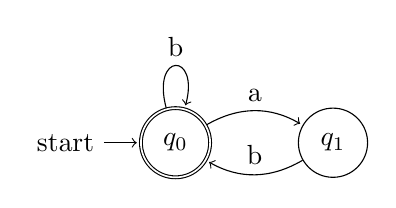
\begin{tikzpicture}[shorten >=1pt,node distance=2cm,on grid,auto]
     \node[state,initial,accepting] (q_0)   {$q_0$};
     \node[state] (q_1) [right=of q_0]  {$q_1$};
      \path[->]
      (q_0) edge [loop above] node  {b} ()
            edge [bend left]  node [above] {a} (q_1)
      (q_1) edge [bend left]  node [above] {b} (q_0);
  \end{tikzpicture}
  \end{center}
  This NFA shows us that the language is regular.
  \item The language is not regular, because using the languages that have been shown in the lecture, we know that the language $a^nb^n$ is not regular. So a language which has $a^p b^p$ where $p \in \mathbb{N}$ as a part of the word is also non-regular.
  \item The language is not regular, because the complement of this language contains the language where n = m which is known as $a^n b^n$ from the lecture and known as not regular. If $L_3$ would be regular, then the complement should also be a regular language.
\end{enumerate}

\section*{Exercise 2}
\begin{enumerate}[label= \alph*)]
%L = {a^m b^n | m, n ∈ N, n < m} Let the loop be in b?
  \item
  If we suppose that L is regular, then the pumping lemma applies to it with a constant k. We let $w = a^{k-1}  b^{k - 2}$. Now $w \in L$ since $k - 2 < k - 1$ and $|w| \geq k$. Now let $w = uvz$ be a decomposition from the pumping lemma. Now $|uv| \leq k$ and $|v| \geq 1$ should hold. Then $u = a^{k - 1}$ and $v = b$. By the pumping lemma, we have $uv^2z \in L$, but $uv^2z = a^{k-1} b^2  b^{k - 3}$.
  Since $k - 1 = 2 + k - 3$ we have that $n \nleq m$ and this means that $uv^2z \notin L$ which shows a contradiction.
  %we have that $uv^2z \notin L$ is a contradiction.
% L = {vca^n | v ∈ {a, b, c}^∗ with |v| < n, for some n ∈ N}
  \item
  If we suppose that L is regular, then the pumping lemma applies to it with a constant k. We let $w = vca^k$ with $|v| = k - 1$. Now $w \in L$ since $|v| < n$ and $|w| \geq k$. Now let $w = xyz$ be a decomposition from the pumping lemma. Now $|xy| \leq k$ and $|y| \geq 1$ should hold. Then $x = v^i$ where $i \in \mathbb{N}$ denotes the length of v in characters and $y = v^{k - 1 - i}$ for $1 \leq i < k$. By the pumping lemma, we have $ux^2z \in L$, but $ux^2z = v^i v^{2(k - 1 - i)} ca^k$. Since $|v| > k$, we have that $ux^2z \notin L$ which is a contradiction.
\end{enumerate}

\end{document}
